\documentclass{article}

\usepackage{float}
\usepackage{graphicx}
\graphicspath{ {figures/} }
\usepackage[margin=1.5in]{geometry}

\renewcommand{\figurename}{Fig}
\renewcommand{\thesection}{S\Roman{section}}
\renewcommand{\thefigure}{S\arabic{figure}}

\title{Supporting Information}
\date{}

\begin{document}
\maketitle		

\setcounter{section}{0}
\setcounter{figure}{0}
\renewcommand{\thesection}{S\Roman{section}}
\renewcommand{\thefigure}{S\arabic{figure}}

\section{Simulated Examples}
\subsection{Trefoil Plots}
For the trefoil example, the signal $Y$ consisted of a trefoil knot embedded in three dimensions containing 500 points. $Z + \epsilon$ was constructed by adding seven superfluous dimensions and isotropic Gaussian noise. Various degrees of noise were tested ($sd = 5, 10, 15, 20, 25, 30$). The first two plots depict Trustworthiness vs. Perplexity and the trustworthiness-maximizing embeddings for the $sd = 10$ case. The third plot shows the trustworthiness-maximizing perplexity for the different degrees of noise.

\begin{figure}[H]
\centering
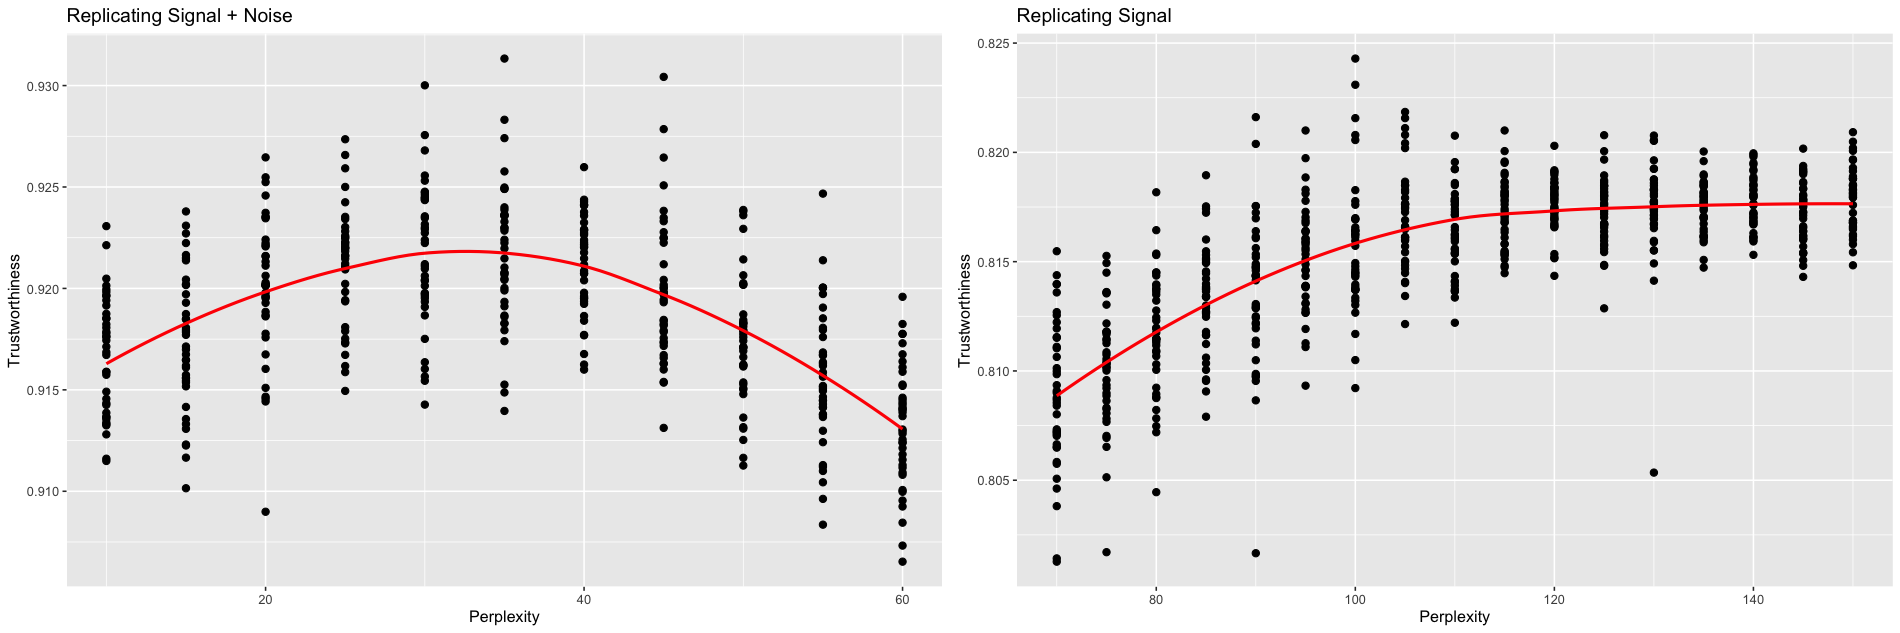
\includegraphics[scale=0.2]{trust_plot_trefoil}
\caption{Trustworthiness vs. Perplexity (Trefoil)}
\end{figure}

\begin{figure}[H]
\centering
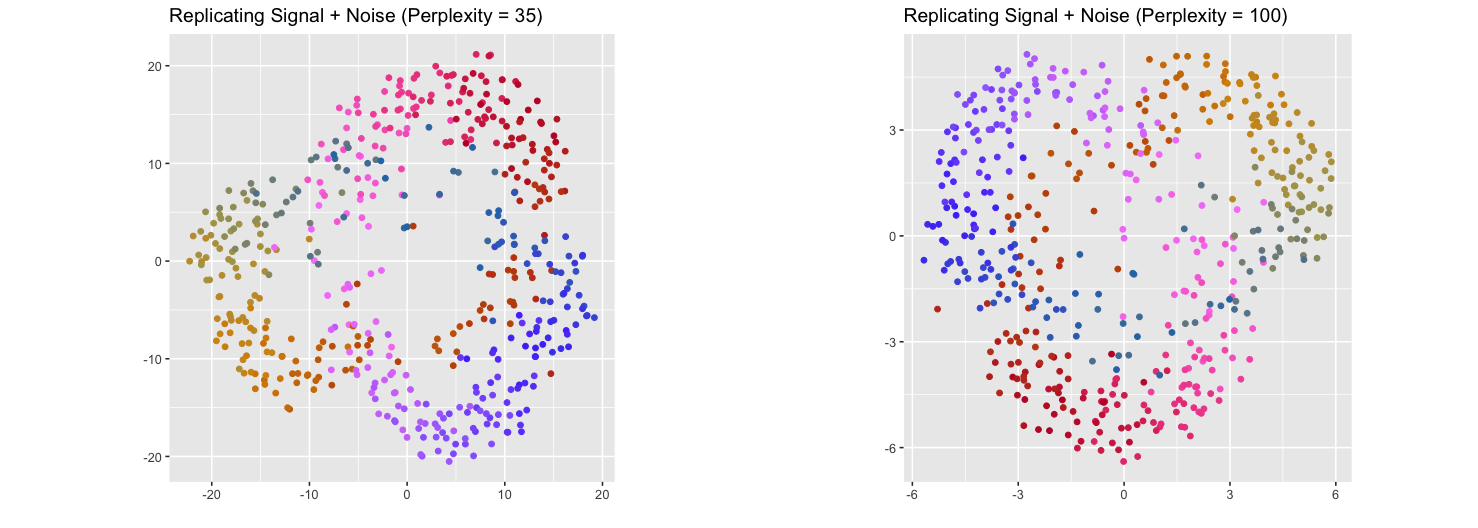
\includegraphics[scale=0.28]{best_rep_trefoil}
\caption{Trustworthiness-Maximizing Representations (Trefoil)}
\end{figure}

\begin{figure}[H]
\centering
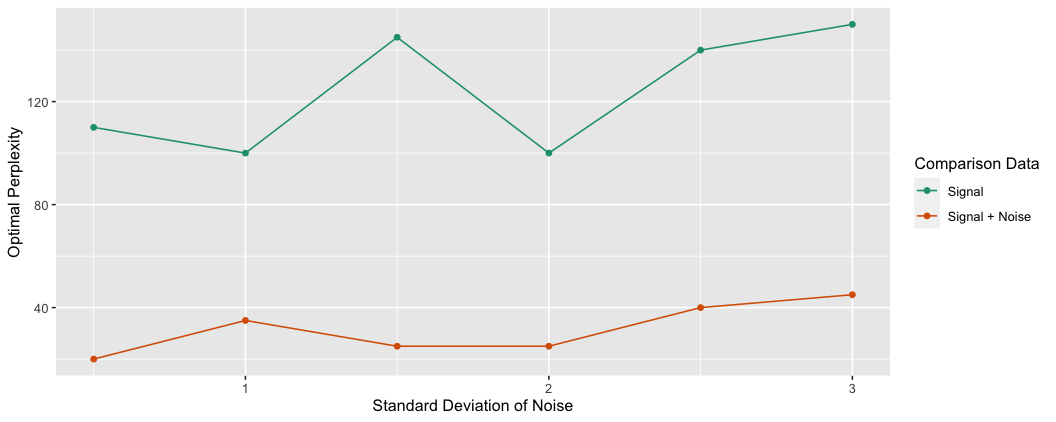
\includegraphics[scale=0.37]{optimal_perp_trefoil}
\caption{Optimal Perplexity (Trefoil)}
\end{figure}

\subsection{Mammoth Plots}
For the mammoth example, the signal $Y$ consisted of 500 points in three dimensions. The data was randomly sampled from the mammoth data set used in \cite{understanding DR}. $Z + \epsilon$ was constructed by adding seven superfluous dimensions and isotropic Gaussian noise. Various degrees of noise were tested ($sd = 0.5, 1, 1.5, 2, 2.5, 3$). The first two plots depict Trustworthiness vs. Perplexity and the trustworthiness-maximizing embeddings for the $sd = 1$ case. The third plot shows the trustworthiness-maximizing perplexity for the different degrees of noise.

\begin{figure}[H]
\centering
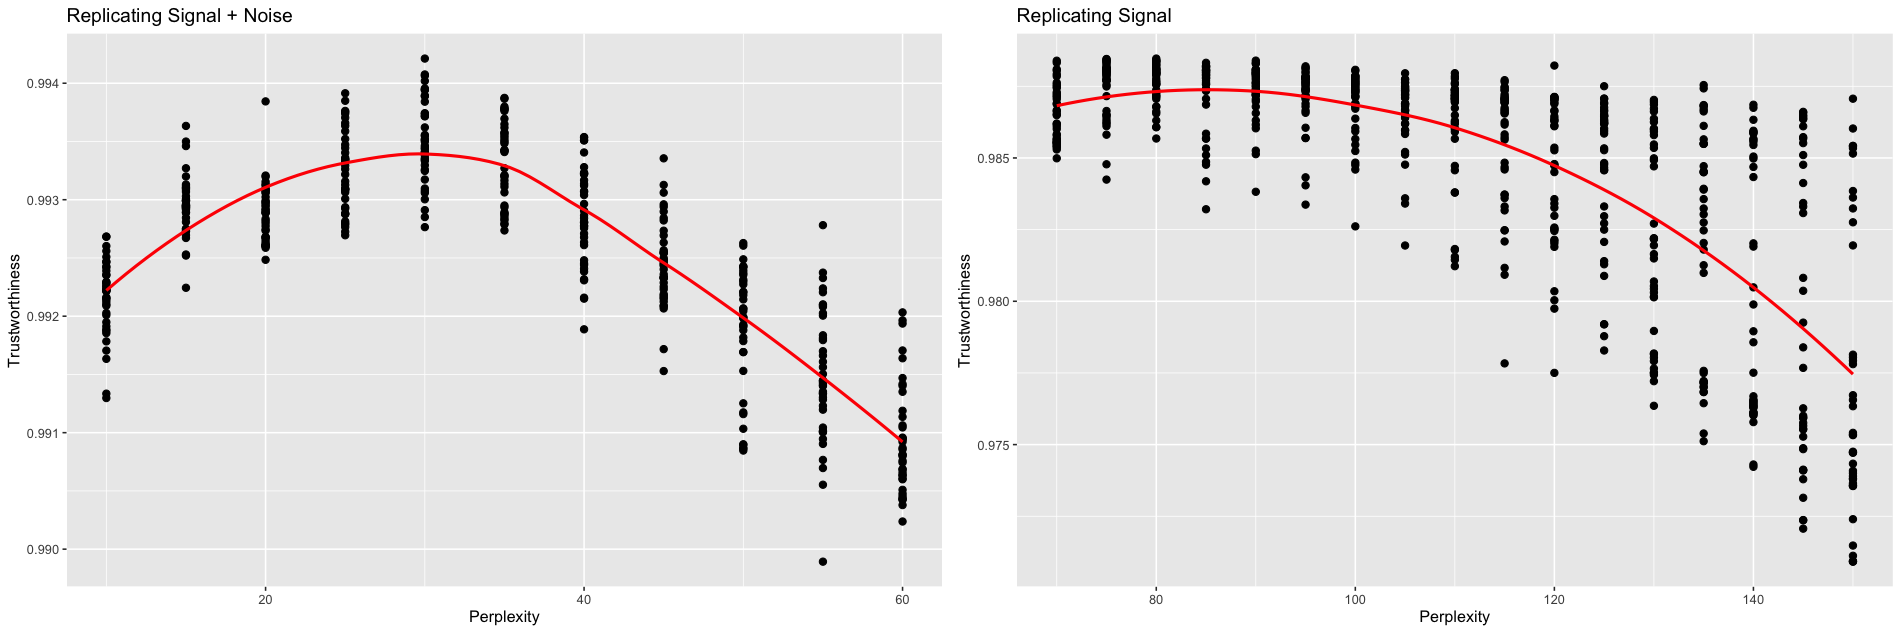
\includegraphics[scale=0.2]{trust_plot_mammoth}
\caption{Trustworthiness vs. Perplexity (Mammoth)}
\end{figure}

\begin{figure}[H]
\centering
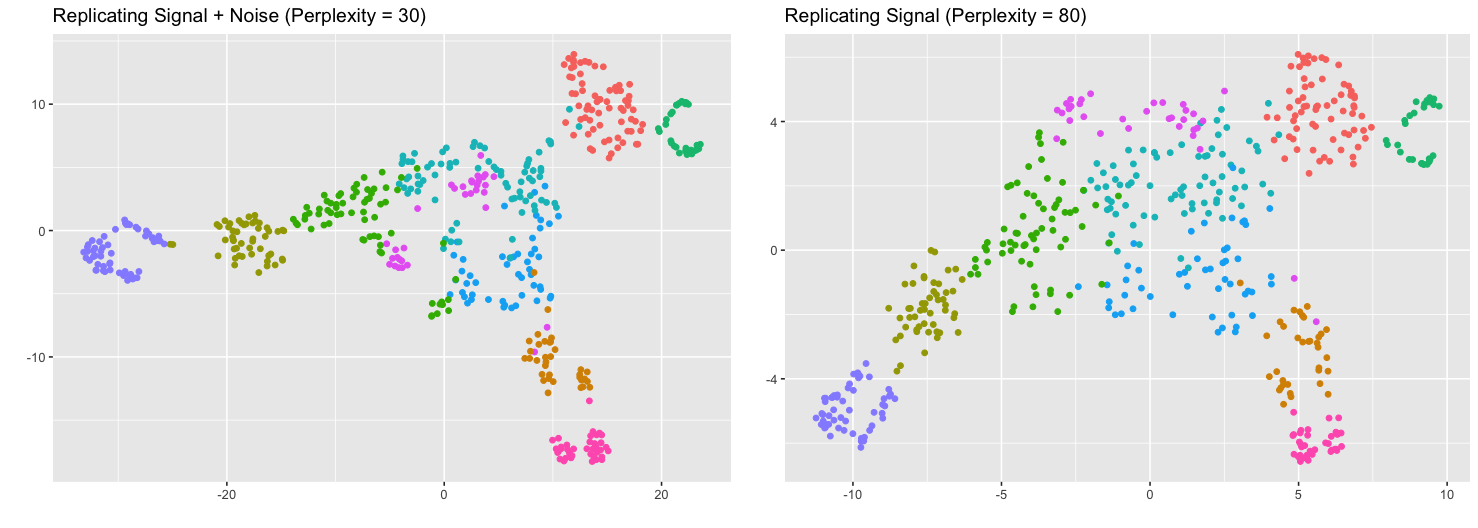
\includegraphics[scale=0.28]{best_rep_mammoth}
\caption{Trustworthiness-Maximizing Representations (Mammoth)}
\end{figure}

\begin{figure}[H]
\centering
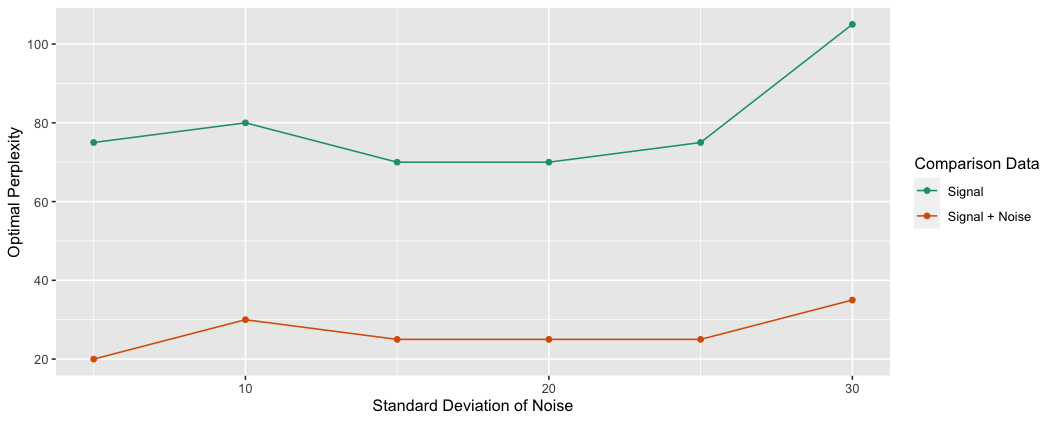
\includegraphics[scale=0.37]{optimal_perp_mammoth}
\caption{Optimal Perplexity (Mammoth)}
\end{figure}

\section{Practical Examples}

\subsection{CyTOF Data Set}
The CyTOF data set contained 239,933 observations in 49 dimensions \cite{CyTOF data}. To reduce the computational load, a subset of 5,000 observations was sampled. A log transformation was followed by a PCA pre-processing step to reduce the number of dimensions to 30, which still retained 77\% of the variance in the original data. The processed data set to be studied consisted of 5,000 observations in 30 dimensions. The signal was first taken to be the first five principal components, then the first eight principal components. A hierarchical clustering of the high-dimensional data was computed then projected onto the trustworthiness-maximizing representations.

\begin{figure}[H]
\centering
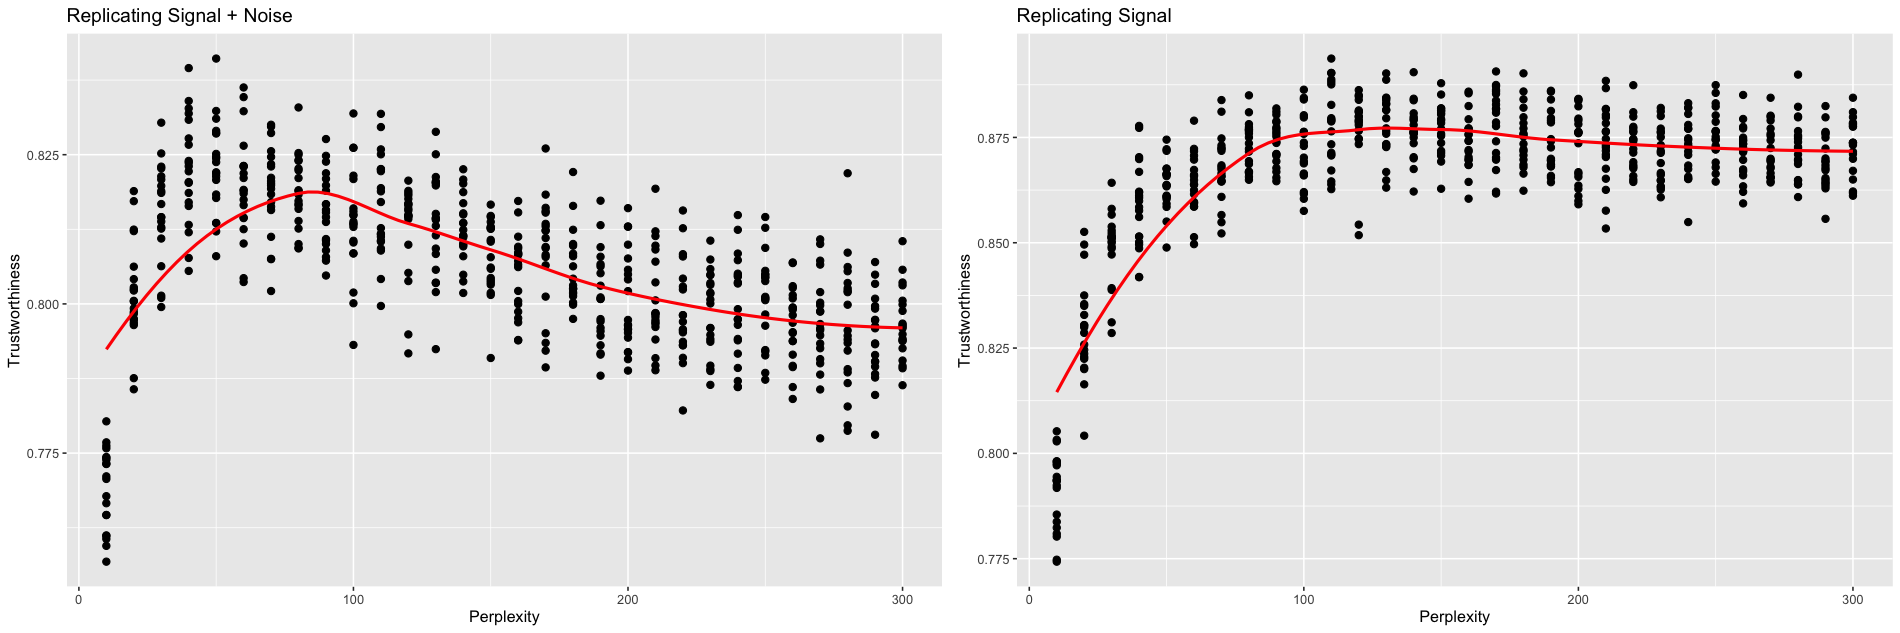
\includegraphics[scale=0.205]{trust_plot_CyTOF}
\caption{Trustworthiness vs. Perplexity for r = 5 (CyTOF)}
\end{figure}

\begin{figure}[H]
\centering
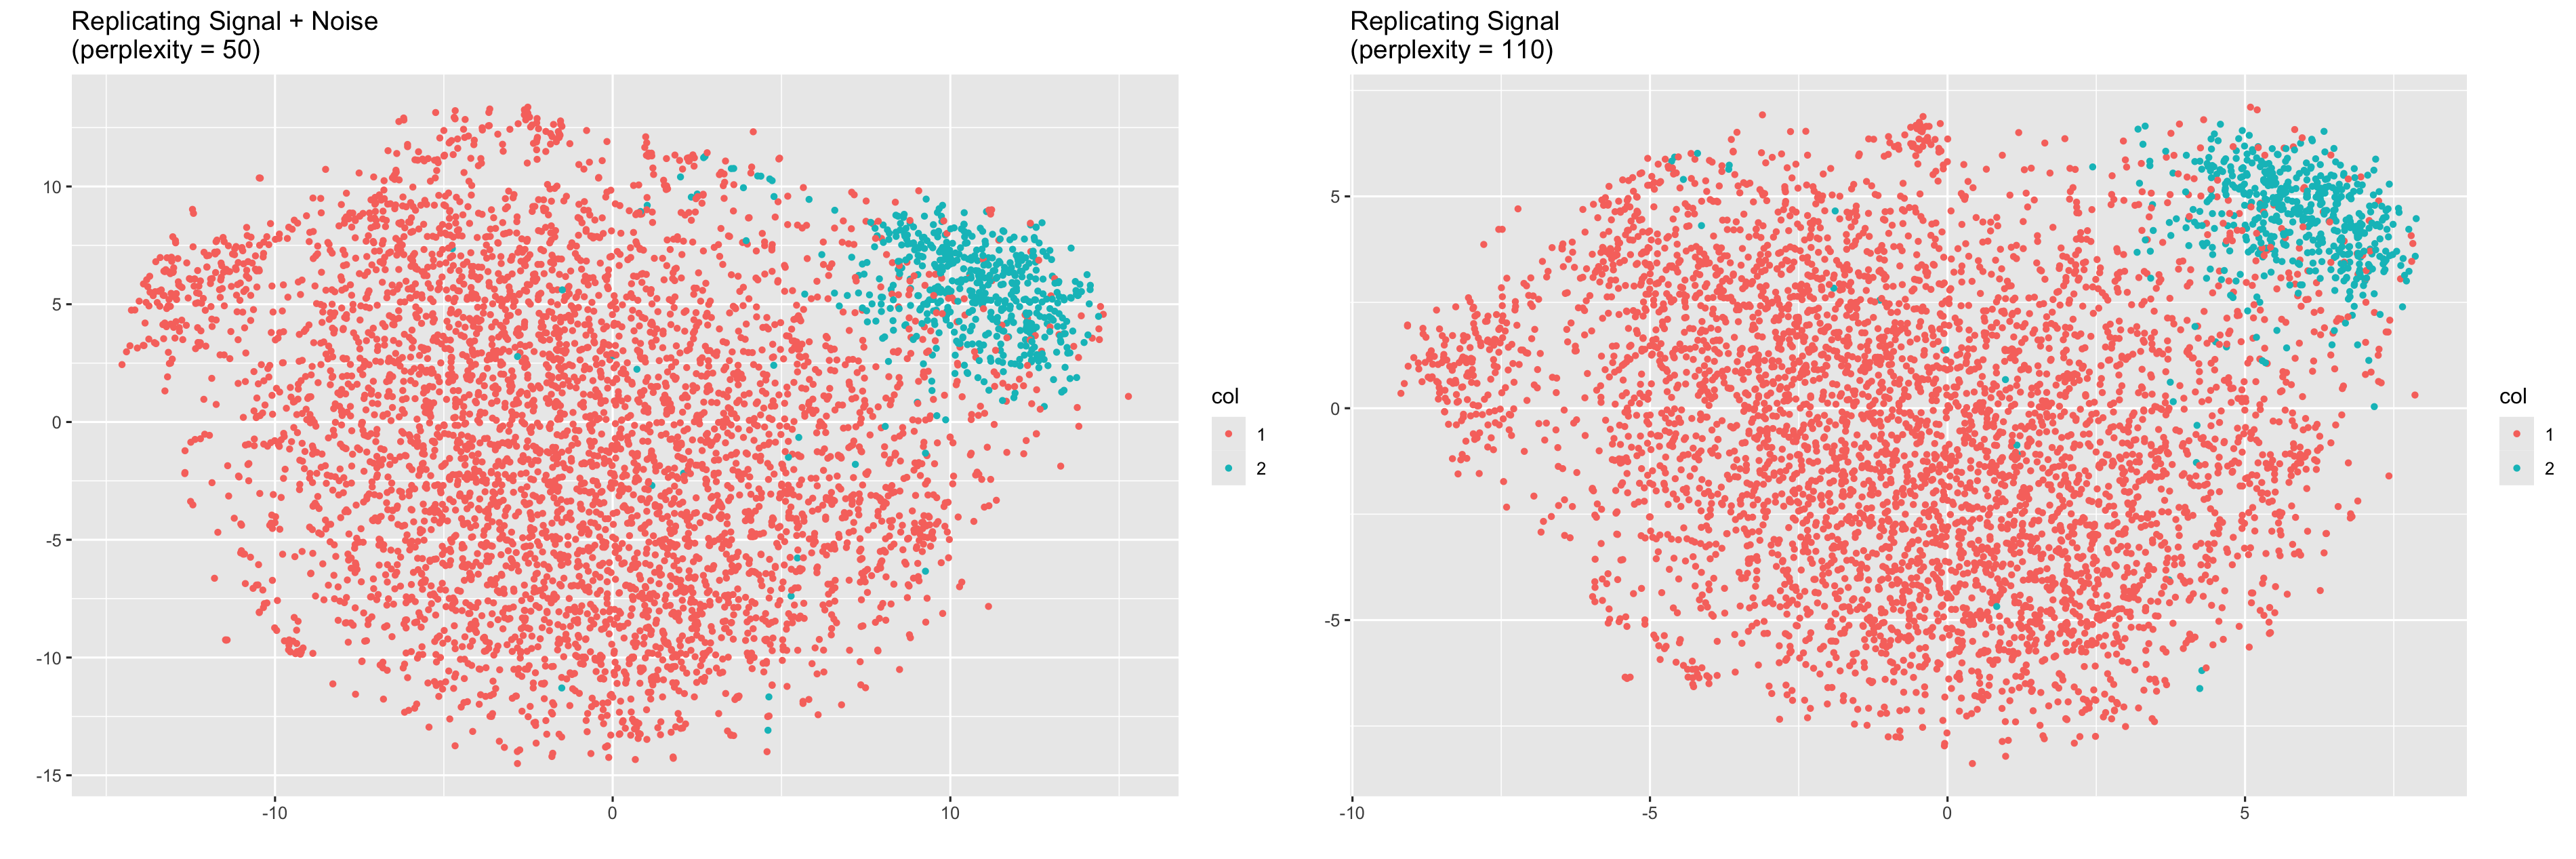
\includegraphics[scale=0.102]{best_rep_CyTOF}
\caption{Trustworthiness-Maximizing Representations for r = 5 (CyTOF)}
\end{figure}

\begin{figure}[H]
\centering
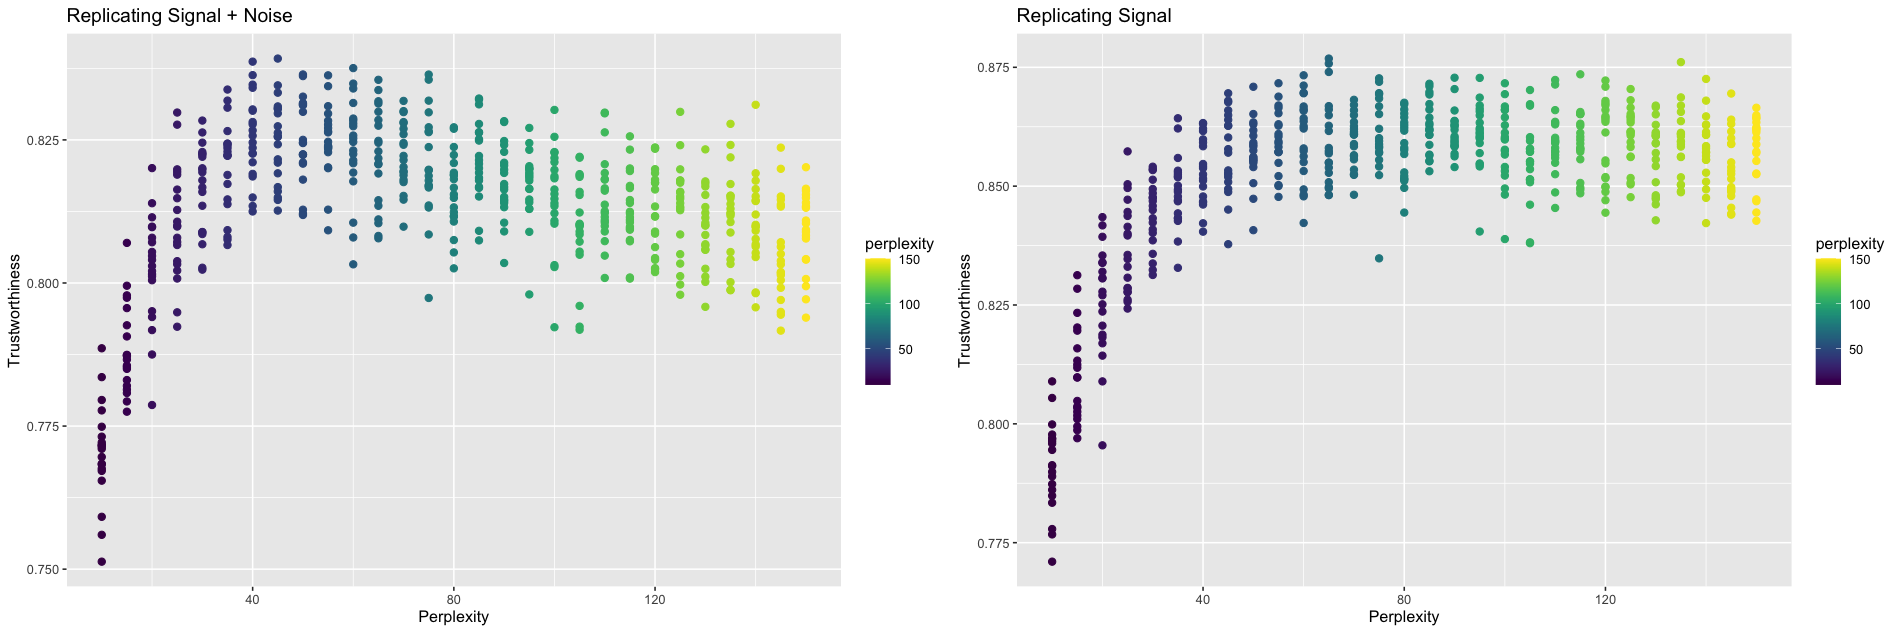
\includegraphics[scale=0.205]{trust_plot_CyTOF2}
\caption{Trustworthiness vs. Perplexity for r = 8 (CyTOF)}
\end{figure}

\begin{figure}[H]
\centering
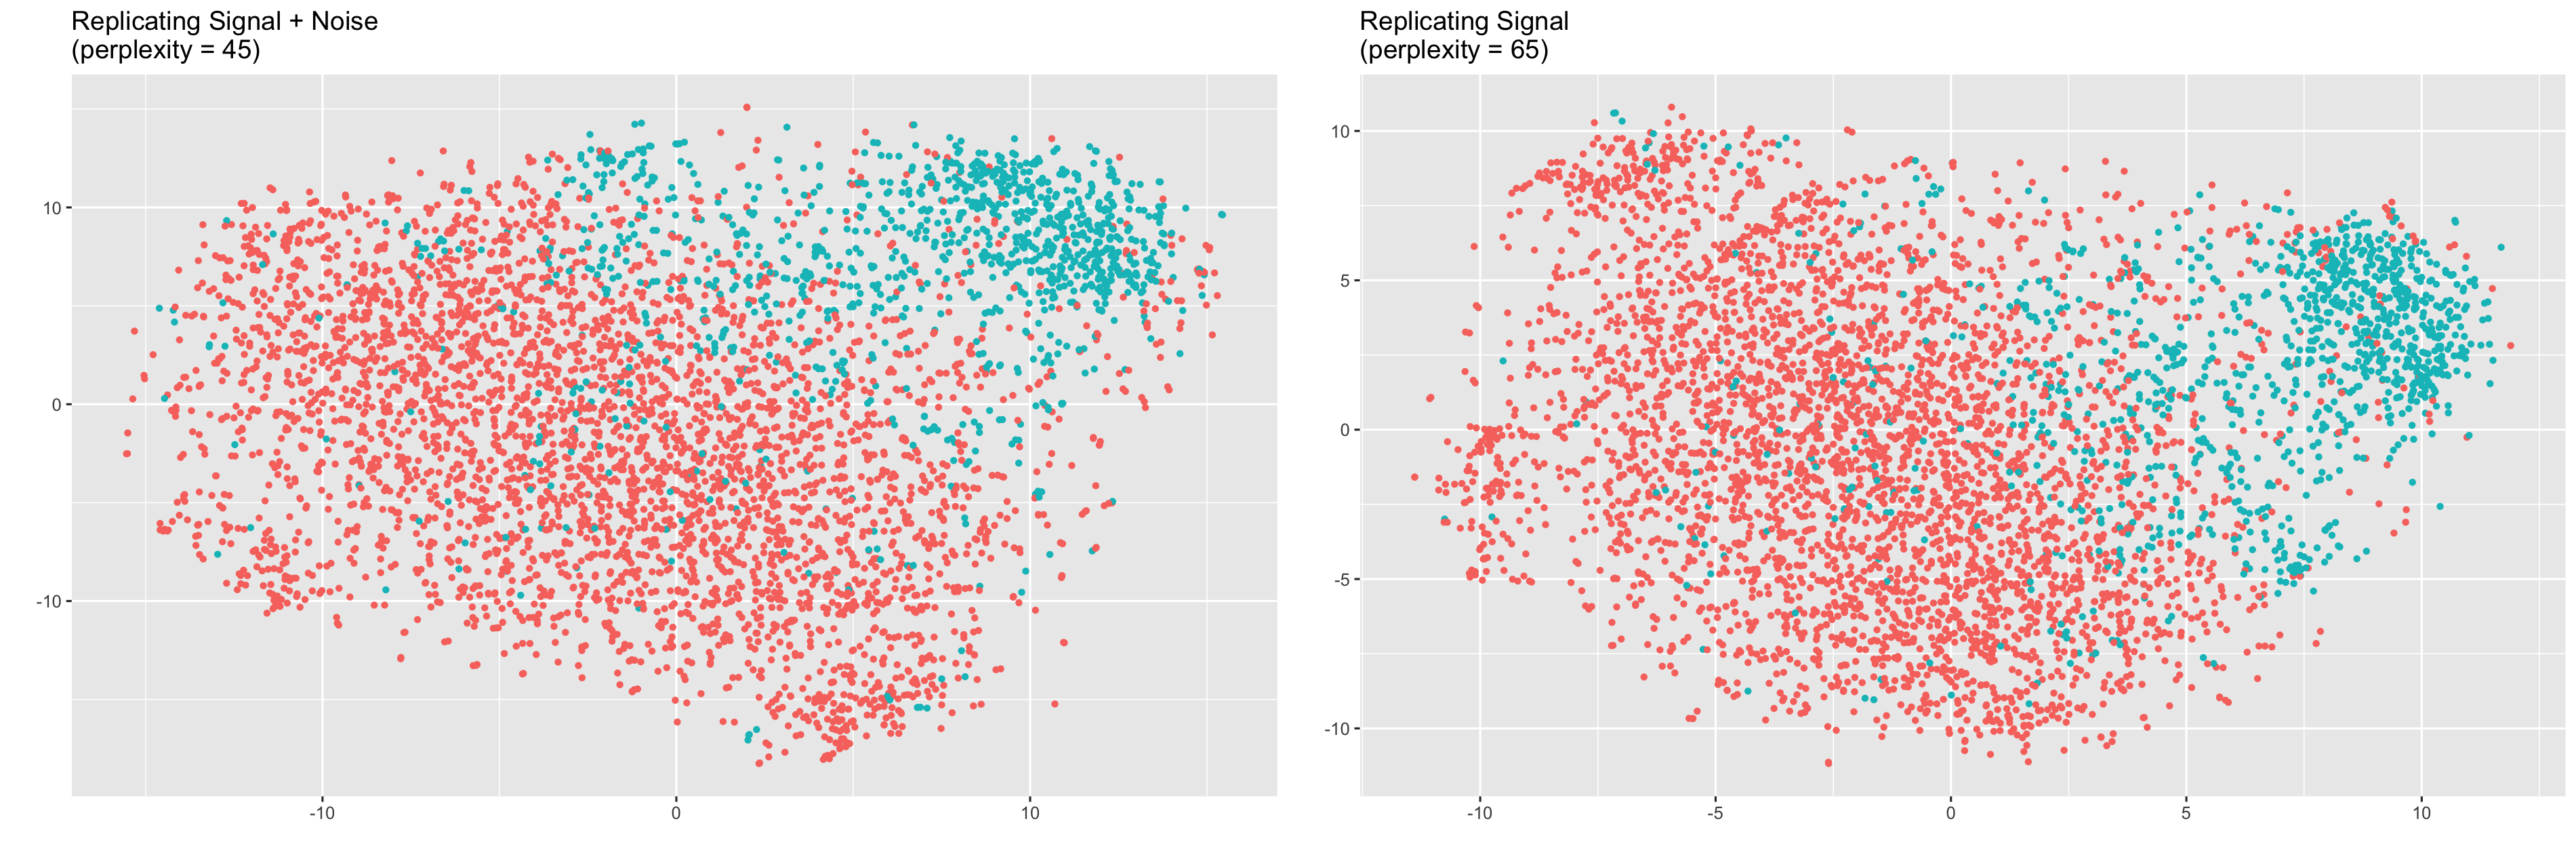
\includegraphics[scale=0.102]{best_rep_CyTOF2}
\caption{Trustworthiness-Maximizing Representations for r = 8 (CyTOF)}
\end{figure}

\subsection{Microbiome Data Set}
\cite{enterotype data} compares the faecal microbial communities from 22 subjects using complete shotgun DNA sequencing. The original data contained 280 samples and 553 genera. To deal with a large number of near-zero readings, columns containing a large proportion of values less than $10^{-6}$ (60\% or more) were removed. This reduced the dimension to 66. A PCA pre-processing was used to center and re-scale the data. The signal was first taken to be the first five principal components, then the first eight principal components. A k-means clustering of the high-dimensional data was computed then projected onto the trustworthiness-maximizing representations.

\begin{figure}[H]
\centering
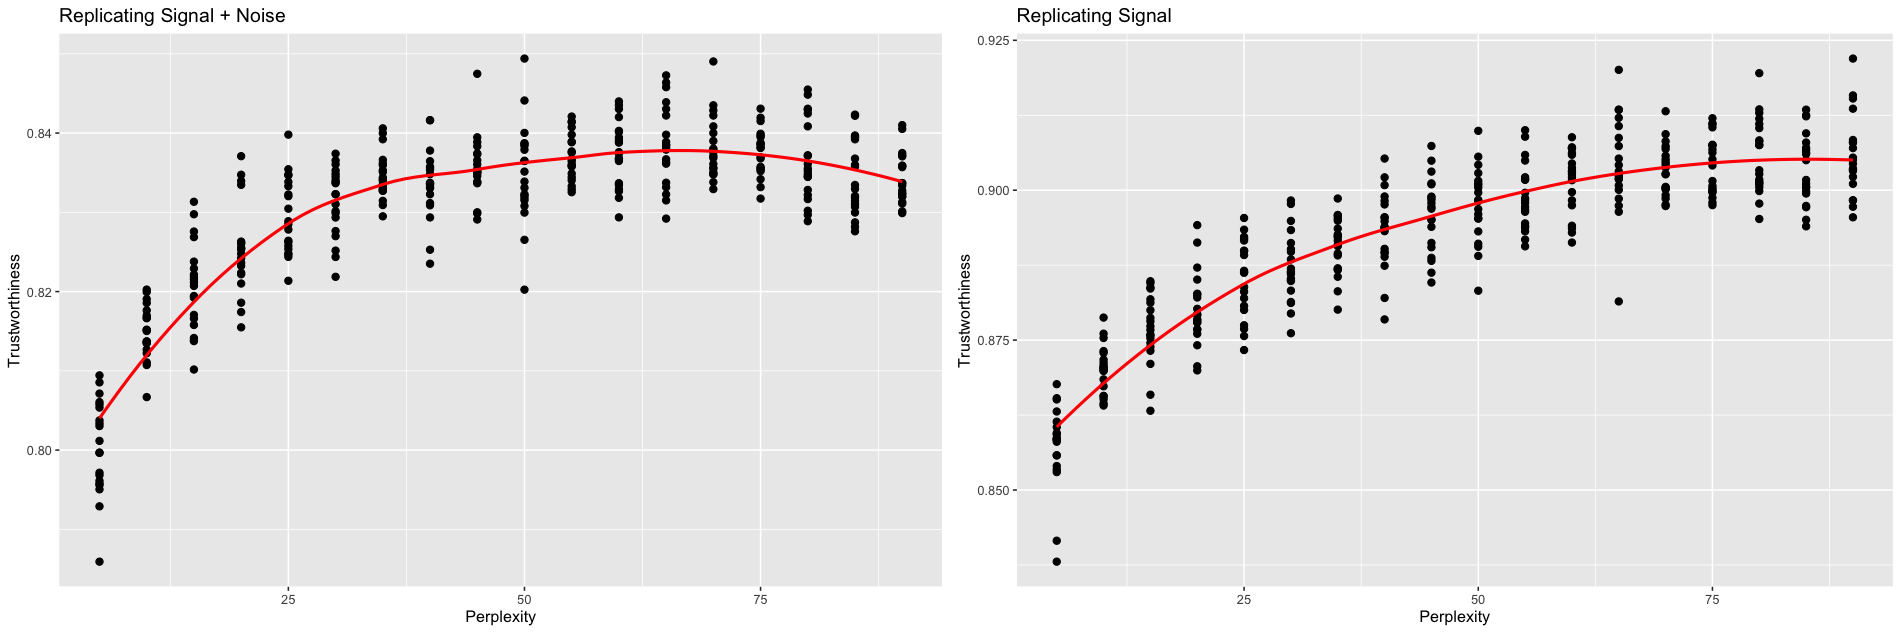
\includegraphics[scale=0.205]{trust_plot_enterotype}
\caption{Trustworthiness vs. Perplexity for r = 5 (Microbiome)}
\end{figure}

\begin{figure}[H]
\centering
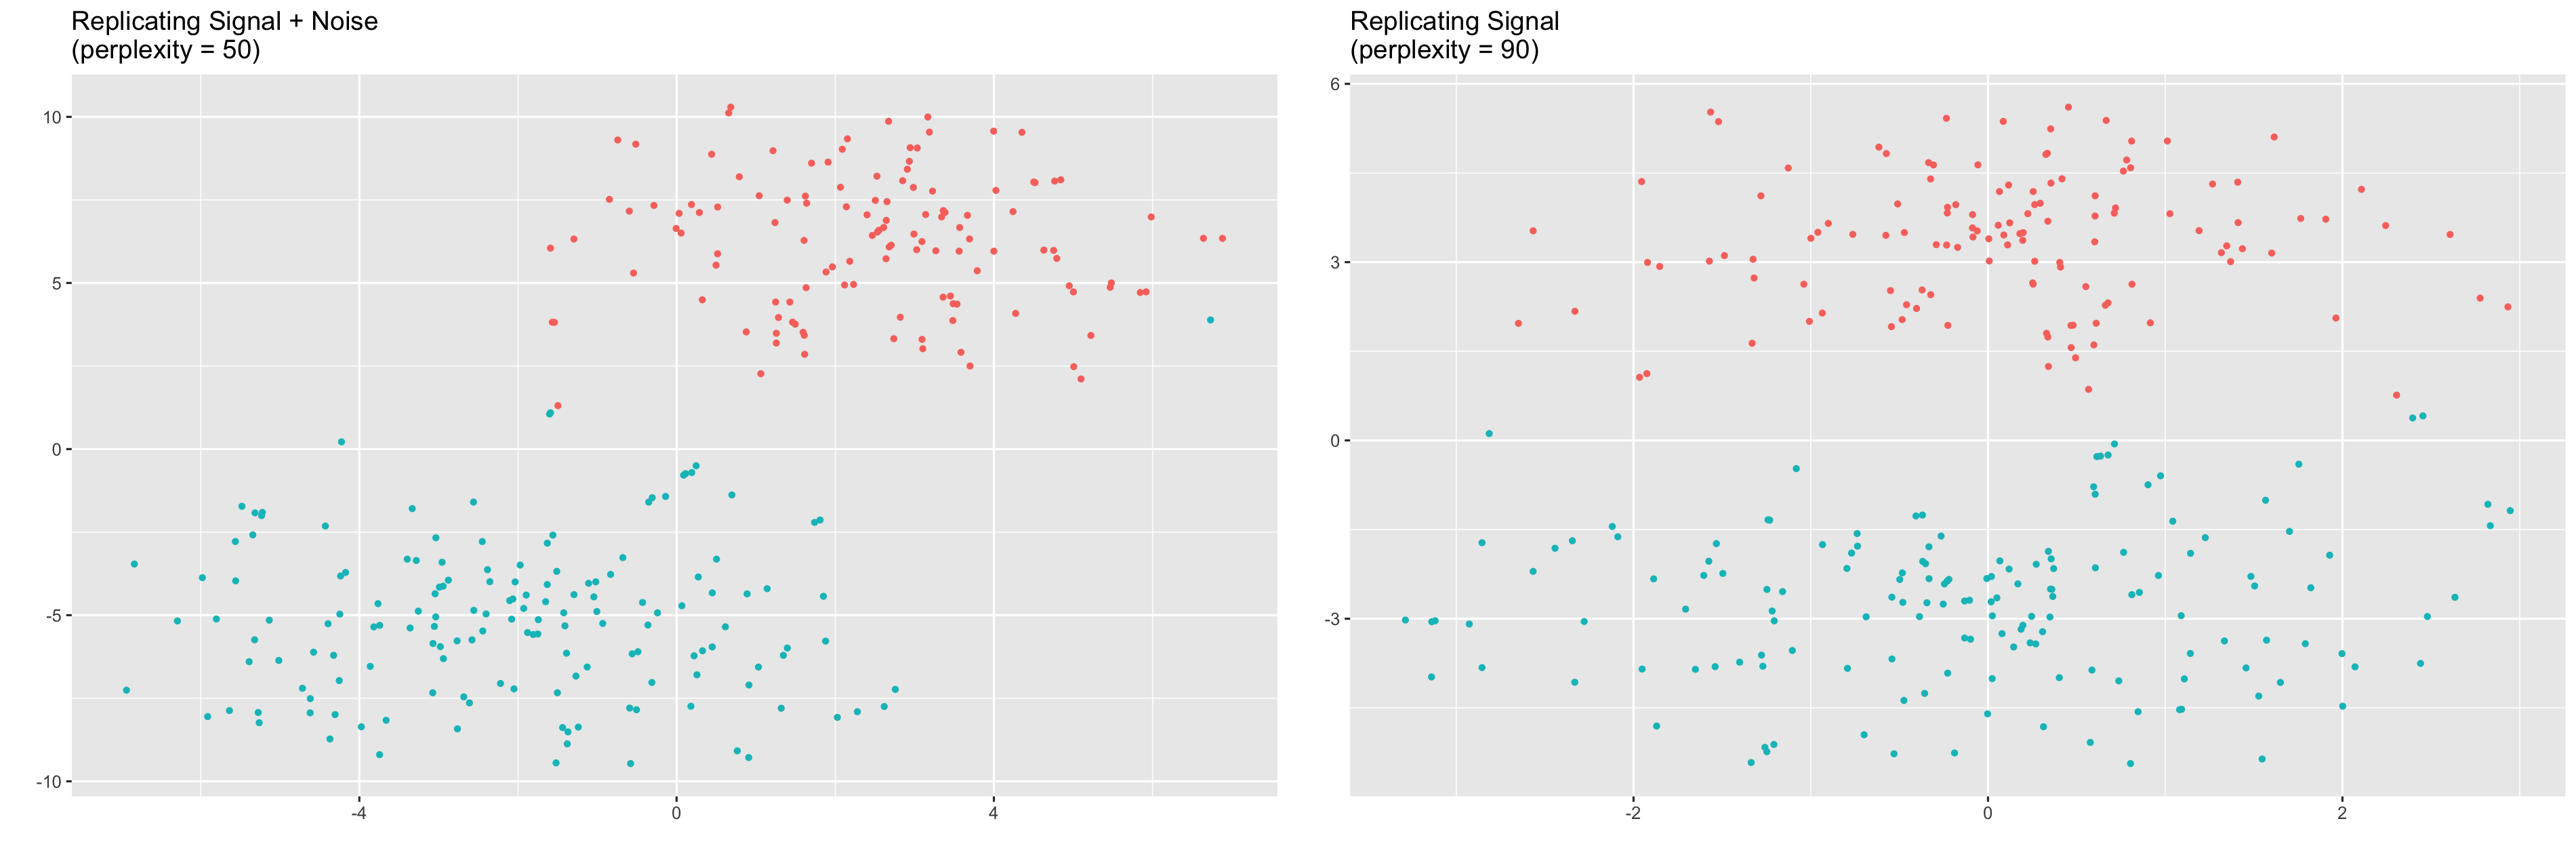
\includegraphics[scale=0.102]{best_rep_enterotype}
\caption{Trustworthiness-Maximizing Representations for r = 5 (Microbiome)}
\end{figure}

\begin{figure}[H]
\centering
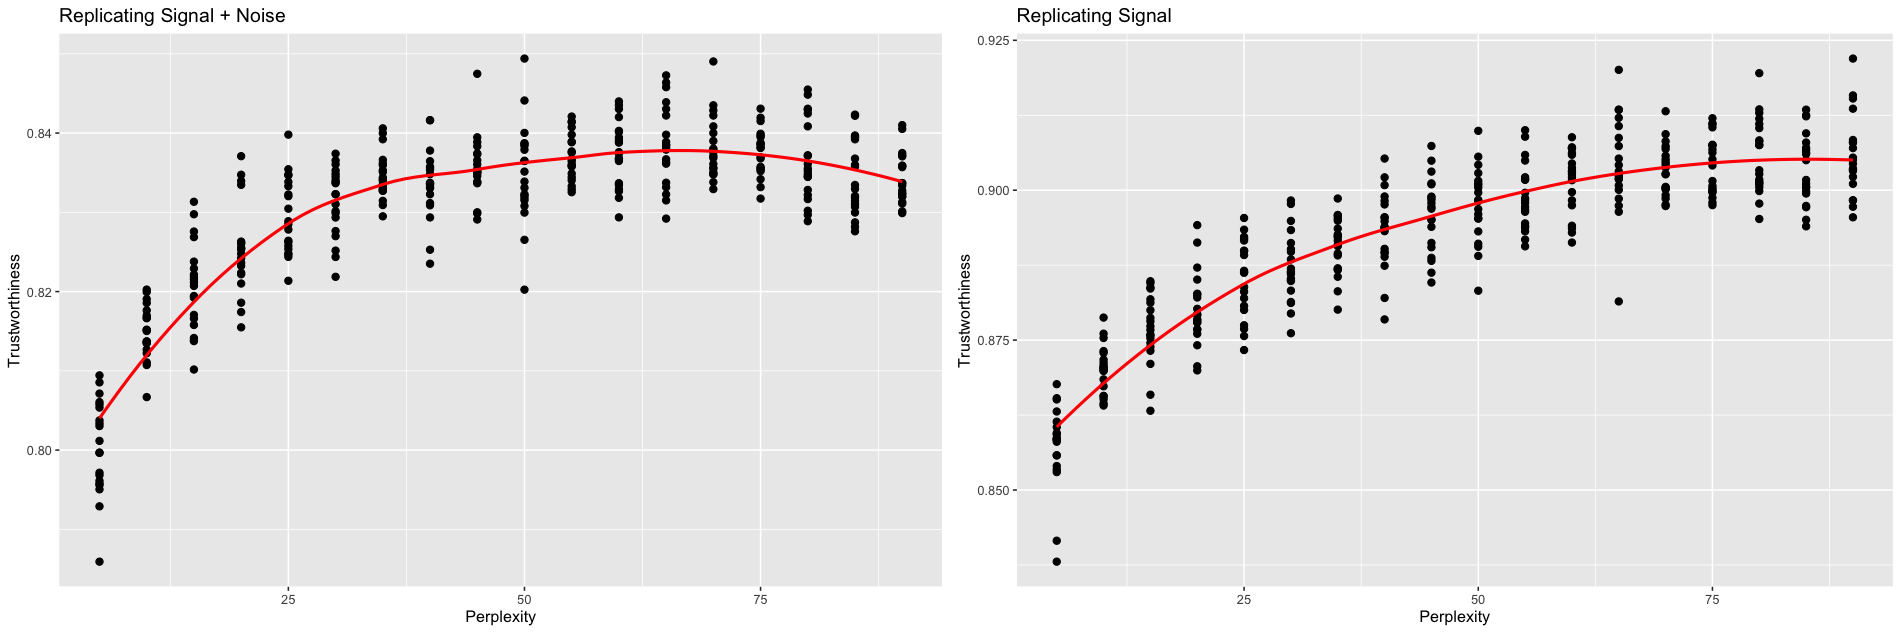
\includegraphics[scale=0.205]{trust_plot_enterotype}
\caption{Trustworthiness vs. Perplexity for r = 8 (Microbiome)}
\end{figure}

\begin{figure}[H]
\centering
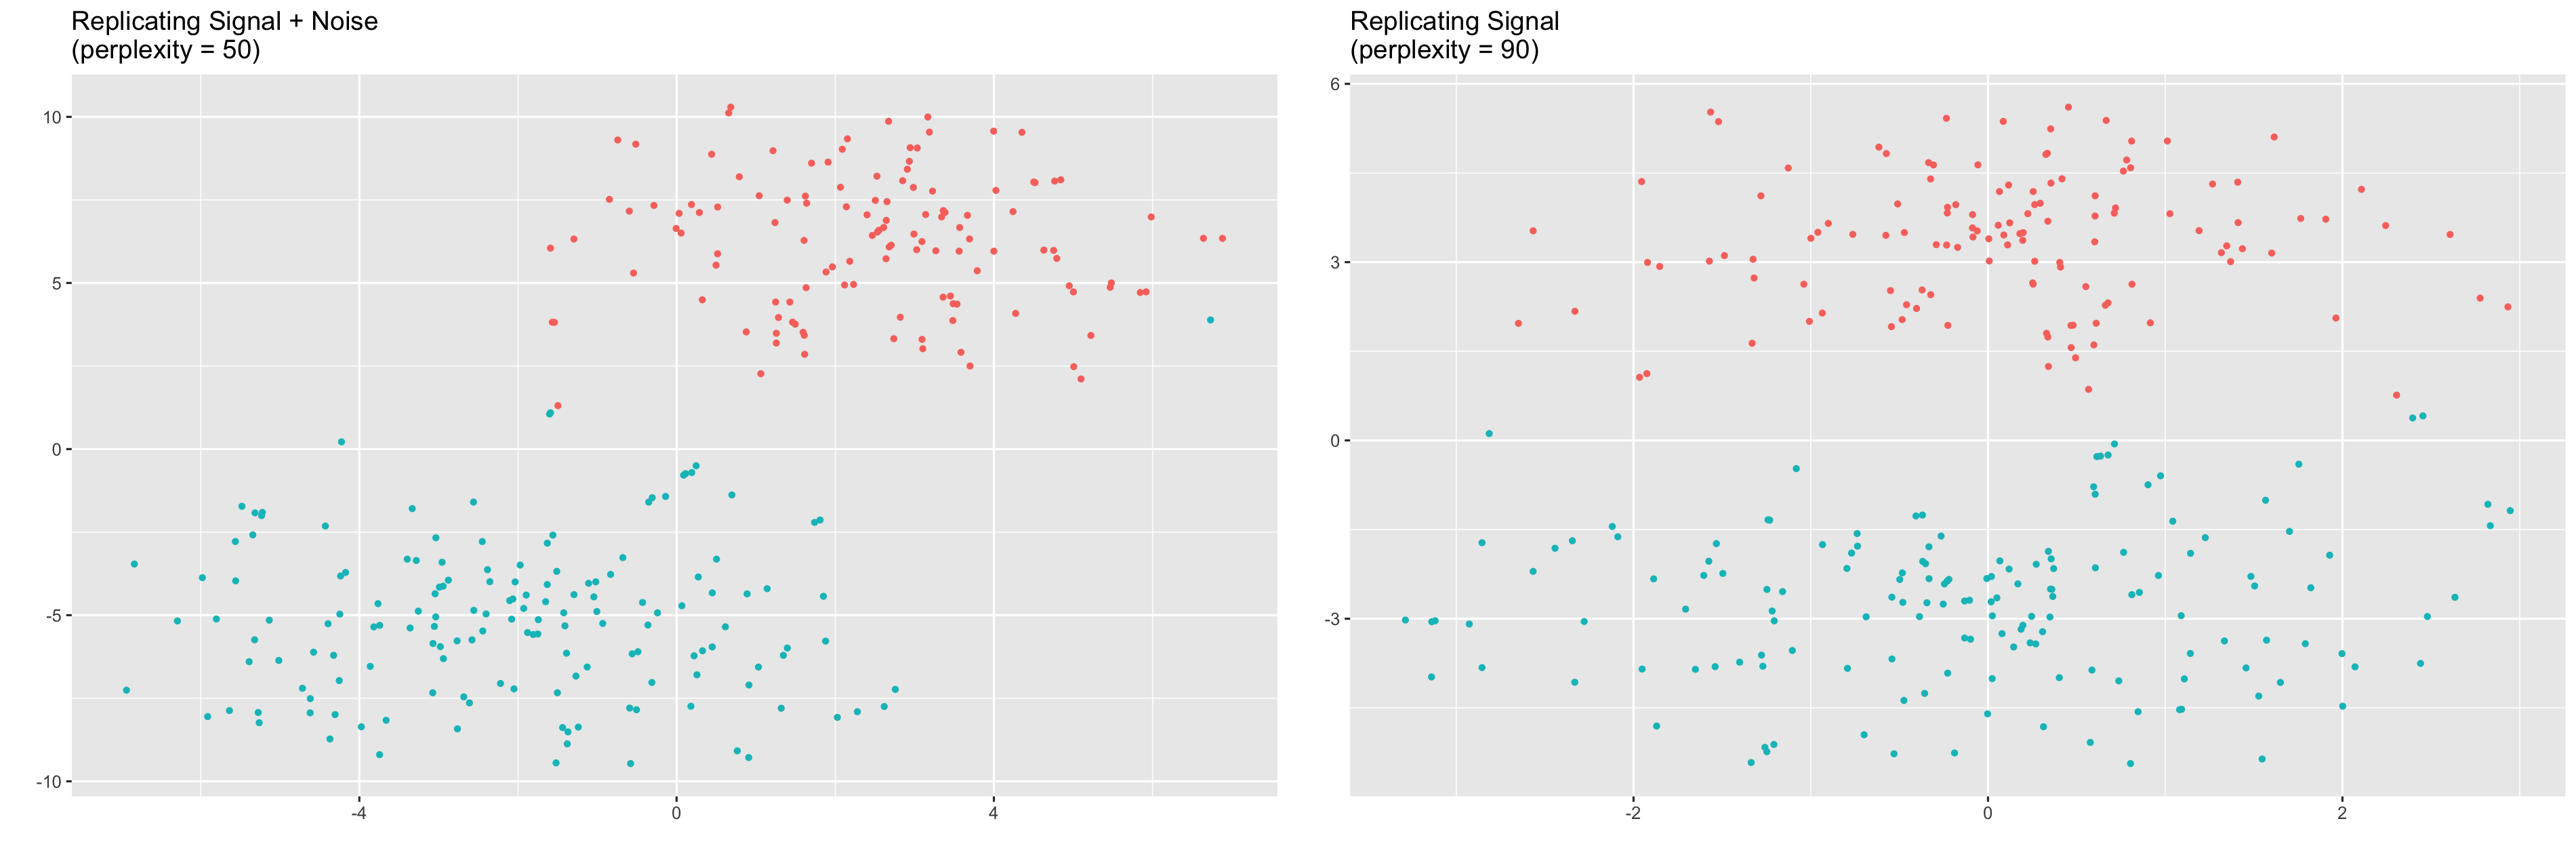
\includegraphics[scale=0.102]{best_rep_enterotype}
\caption{Trustworthiness-Maximizing Representations for r = 8 (Microbiome)}
\end{figure}

\section{PBMC Data Set}

\begin{figure}[H]
\centering
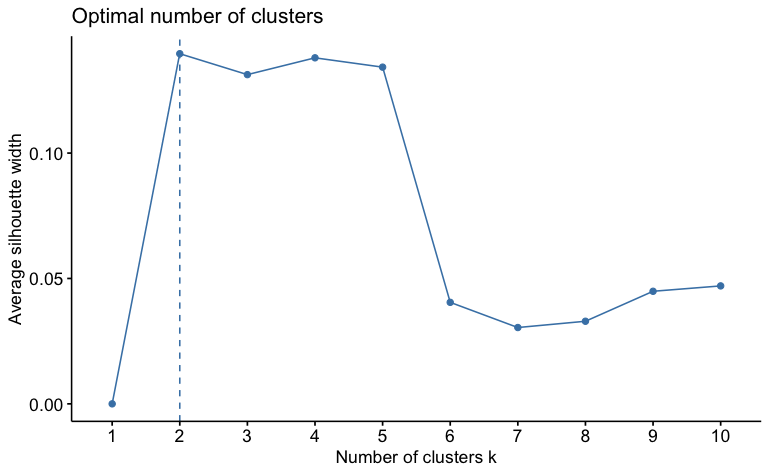
\includegraphics[scale=0.35]{BPCells_silhouette}
\caption{Average Silhouette Width for Dendritic Cells}
\end{figure}

\begin{figure}[H]
\centering
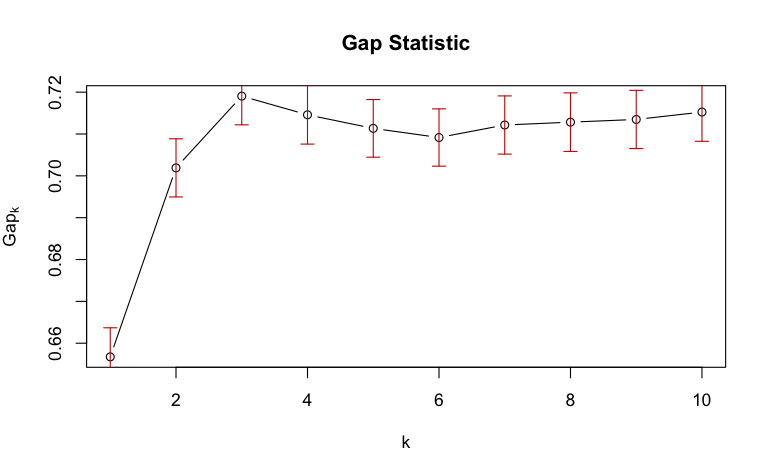
\includegraphics[scale=0.35]{BPCells_gap}
\caption{Gap Statistic for Dendritic Cells}
\end{figure}

\newpage
\bibliographystyle{abbrvnat}
\bibliography{reference}

\begin{thebibliography}{10}

\bibitem{t-SNE example}
Amir et al.
\newblock viSNE enables visualization of high dimensional single-cell data and reveals phenotypic heterogeneity of leukemia.
\newblock {\em Nature Biotechnology 31 545-552}, 2013.

\bibitem{SVD example}
Orly Alter, Patrick O. Brown, and David Botstein.
\newblock Singular value decomposition for genome-wide expression data processing and modeling.
\newblock {\em PNAS 97(18) 10101-10106}, 2000.

\bibitem{PHATE}
Moon et al.
\newblock Visualizing structure and transitions in high-dimensional biological data.
\newblock {\em Nat Biotechnology 37(12):1482-1492}, 2019.

\bibitem{t-SNE}
Laurens van der Maaten and Geoffrey Hinton.
\newblock Visualizing data using t-SNE.
\newblock {\em Journal of Machine Learning Research 9:2579 -- 2605}, 2008.

\bibitem{umap}
Leland McInnes, John Healy, and James Melville.
\newblock UMAP: Uniform Manifold Approximation and Projection for dimension reduction.
\newblock {\em arXiv preprint arXiv:1802.03426v3}, 2020.

\bibitem{UMAP example}
Becht et al.
\newblock Dimensionality reduction for visualizing single-cell data using UMAP.
\newblock {\em Nature Biotechnology 37 38-44}, 2019.

\bibitem{t-SNE/UMAP example}
Dmitry Kobak and George C. Linderman.
\newblock Initialization is critical for preserving global data structure in both t-SNE and UMAP.
\newblock {\em Nature Biotechnology 39 156-157}, 2021.

\bibitem{perplexity-free t-SNE}
Francesco Crecchi, Cyril de Bodt, Michel Verleysen, John A. Lee, and Davide Bacciu.
\newblock Perplexity-free parametric t-SNE.
\newblock {\em arXiv preprint arXiv:2010.01359v1}, 2020.

\bibitem{evaluation of DR transcriptomics}
Haiyang Huang, Yingfan Wang, Cynthia Rudin, and Edward P. Browne.
\newblock Towards a comprehensive evaluation of dimension reduction methods for transcriptomic data visualization.
\newblock {\em Communications Biology, 5:716}, 2022.

\bibitem{t-SNE cell}
Dmitry Kobak and Philipp Berens.
\newblock The art of using t-SNE for single-cell transcriptomics.
\newblock {\em Nature Communications, 10:5416}, 2019.

\bibitem{perplexity vs kl}
Yanshuai Cao and Luyu Wang. 
\newblock Automatic selection of t-SNE perplexity.
\newblock {\em arXiv preprint arXiv:1708.03229.v1}, 2017.

\bibitem{diffusion maps}
Ronald R. Coifman and St\'ephane Lagon.
\newblock Diffusion maps.
\newblock {\em Applied and Computational Harmonic Analysis 21:1 5-30}, 2006.

\bibitem{Distill}
Martin Wattenberg, Fernanda Vi\'egas, and Ian Johnson.
\newblock How to Use t-SNE Effectively.
\newblock {\em Distill}, 2016.

\bibitem{understanding UMAP}
Andy Coenen and Adam Pearce for Google PAIR.
\newblock Understanding UMAP.
\newblock {\em https://pair-code.github.io/understanding-umap/}.

\bibitem{large DR unreliable}
Tara Chari and Lior Pachter.
\newblock The specious art of single-cell genomics.
\newblock {\em PLoS Computational Biology 19(8):e1011288},  2023.

\bibitem{quantitative survey}
Mateus Espadoto, Rafael M. Martins, Andreas Kerren, Nina S. T. Hirata, and Alexandru C. Telea.
\newblock Towards a quantitative survey of dimension reduction techniques.
\newblock {\em IEEE Transactions on Visualization and Computer Graphics 27:3}, 2021.

\bibitem{trustworthiness}
Jarkko Venna and Samuel Kaski.
\newblock Visualizing gene interaction graphs with local multidimensional scaling.
\newblock {\em European Symposium on Artificial Neural Networks}, 2006.

\bibitem{understanding DR}
Yingfan Wang, Haiyang Huang, Cynthia Rudin, and Yaron Shaposhnik.
\newblock Understanding how dimension reduction tools work: An empirical approach to deciphering t-SNE, UMAP, TriMap, and PaCMAP for data visualization.
\newblock {\em Journal of Machine Learning Research 22}, 2021.

\bibitem{Rtsne}
Jesse H. Krijthe.
\newblock Rtsne: T-Distributed Stochastic Neighbor Embedding using a Barnes-Hut Implementation.
\newblock {\em https://github.com/jkrijthe/Rtsne}, 2015.

 \bibitem{scRNA data}
 Po-Yuan Tung, John D. Blischak, Chiaowen Joyce Hsiao, David A. Knowles, Jonathan E. Burnett, Jonathan K. Pritchard, et al.
 \newblock Batch effects and the effective design of single-cell gene expression studies.
 \newblock {\em Scientific Reports 7:39921}, 2017.

\bibitem{CyTOF data}
Dara M. Strauss-Albee, Julia Fukuyama, Emily C. Liang, Yi Yao, Justin A. Jarrell, Alison L. Drake, et al.
\newblock Human NK cell repertoire diversity reflects immune experience and correlates with viral susceptibility.
\newblock {\em Science Translational Medicine 7:297}, 2015.

\bibitem{enterotype data}
Manimozhiyan Arumugam, Jeroen Raes, Eric Pelletier, Denis Le Paslier, Takuji Yamada, Daniel R. Mende, et al.
\newblock Enterotypes of the human gut microbiome.
\newblock {\em Nature 473 174-180}, 2011.

\bibitem{parallel analysis}
Horn, John L.
\newblock A rationale and test for the number of factors in factor analysis.
\newblock {\em Psychometrika 30:2 179-185}, 1965.

\bibitem{subsample t-SNE}
Martin Skrodzki, Nicolas Chaves-de-Plaza, Klaus Hildebrandt, Thomas H\"ollt, and Elmar Eisemann.
\newblock Tuning the perplexity for and computing sampling-based t-SNE embeddings.
\newblock {\em arXiv preprint arXiv:2308.15513v1}, 2023.

\bibitem{BPCells data}
Cell Ranger ARC 2.0.0.
\newblock Single Cell Multiome ATAC + Gene Expression Dataset.
\newblock {\em https://www.10xgenomics.com/datasets/pbmc-from-a-healthy-donor-granulocytes-removed-through-cell-sorting-3-k-1-standard-2-0-0}, 2021.

\bibitem{BPCells tutorial}
Benjamin Parks.
\newblock BPCells: Single Cell Counts Matrices to PCA.
\newblock {\em https://bnprks.github.io/BPCells/articles/pbmc3k.html}, 2023.

\bibitem{noise in single-cell data}
Shih-Kai Chu, Shilin Zhao, Yu Shyr, and Qi liu.
\newblock Comprehensive evaluation of noise reduction methods for single-cell RNA sequencing data.
\newblock {\em Briefings in Bioinformatics 23:2}, 2022.

\bibitem{TriMap}
Ehsan Amid and Manfred K. Warmuth. 
\newblock TriMap: Large-scale dimensionality reduction using triplets. 
\newblock {\em arXiv preprint arXiv:1910.00204v2}, 2022.

\bibitem{rank-based criteria}
John A. Lee and Michel Verleysen.
\newblock Quality assessment of dimensionality reduction: Rank-based criteria.
\newblock {\em Neurocomputing 72:1431 -- 1443}, 2009.

\bibitem{precision score}
Tobias Schreck, Tatiana von Landesberger, and Sebastian Bremm.
\newblock Techniques for precision-based visual analysis of projected data.
\newblock {\em Sage 9:3}, 2012.

\end{thebibliography}

\end{document}
